\chapter{Workload Metrics} \label{ch:workload}

Now that we have a basic understanding of the data that the simulator has access to during the simulation we can now discuss how we translate this data into meaningful metrics.  We will first discuss our baseline workload metric.  Afterwards we will describe the two workload metrics we created as part of this work.

\section{Adapted Wickens' Metric}
Since we are interested in metrics that reveal human workload we have chosen to replicate Wickens' computational model~\cite{wickens2002multiple}, shown in equations~\ref{eq:wickens_model}-\ref{eq:resource_demand}, using data gathered from the Model Abstraction Framework.  Wickens' model is a measure of resource demand and overlap that has been shown to predict performance degradation, making it a good baseline metric for evaluating consistency with known high workload events and for comparison with the new metrics presented later in the chapter.  

Wickens' computational model is based on the concept of tasks, where a task is some arbitrary unit of activity.  Wickens' model calculates the resource interference between two tasks, a value that is closely related to mental workload~\cite{wickens2002multiple}.  The problem with using this computational model as a metric within the Model Abstraction Framework is the difference in the modeling paradigms.  In this work we abstract the notion of a task, relying instead on states and transitions to infer activity.  The challenge is to apply the task-based abstraction of Wickens' model to the state/transition based abstraction of the Model Abstraction Framework.

\begin{equation}
  W_{Wickens}(T_{1}, T_{2}) = R_{Demand}(T^{1}, T^{2}) + R_{Conflict}(T^{1}, T^{2})
  \label{eq:wickens_model}
\end{equation}

\begin{equation}
  R_{Demand}(T^{1}, T^{2}) = T_{demand}^{1} + T_{demand}^{2}
  \label{eq:resource_demand}
\end{equation}

\begin{equation}
  R_{Conflict}(T^{1}, T^{2}) = \sum_{x=1}^{dimensions} \left\{
    \begin{array}{l l}
      1 & T_{x}^{1} = T_{x}^{2} \\
      0 & otherwise \\
    \end{array}
    \right.
  \label{eq:resource_conflict}
\end{equation}

Wickens' model $W_{Wickens}$, equation \ref{eq:wickens_model}, calculates the resource interference between two tasks, represented as $T^{1}$ and $T^{2}$, through the use of two components: resource demand $R_{Demand}$ and resource conflict $R_{Conflict}$.  Resource demand is a subjective measure of the cognitive resources required by a task.  In equation \ref{eq:resource_demand} we see that the resource demand of tasks $T^{1}$ and $T^{2}$ is calculated by summing the resource demand of both tasks.  To keep the model simple and intuitive Wickens limits $T_{demand}$ to a range of 0 to 2, where 0 is an automated task and 2 is a difficult task.  Thus $R_{Demand}$ will always be between 0 and 4.


\begin{figure}[h]
\begin{center}
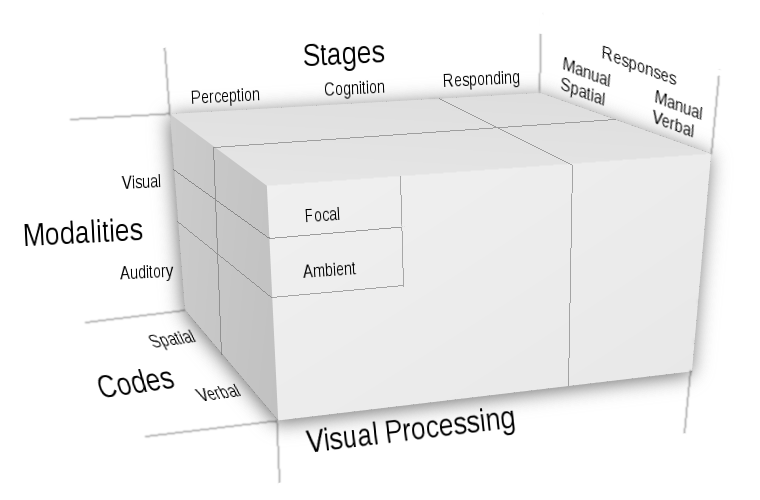
\includegraphics[width=6in]{multipleresourcetheory.png}
\caption{Multiple Resource Theory Dimensions~\cite{wickens2002multiple}}
\label{fig:multipleresourcetheory}
\end{center}
\end{figure}

For resource conflict two tasks are considered to have conflicting resources when they share resources within one of the dimensions illustrated in figure \ref{fig:multipleresourcetheory}.  In equation \ref{eq:resource_conflict} when $T_{x}$ represents the task resources for dimension $x$, then $R_{Conflict}$ is calculated by taking the sum of the total number of resource conflicts between two tasks.  Since there are only four dimensions $R_{Conflict}$ will always be between 0 and 4.  For example if $Task_{A}$ required a person to listen for distinct sounds while $Task_{B}$ required listening to a conversation, the resource conflict would be 2.  One in the {\em Stages} dimension for perception, and another in the {\em Modalities} dimension for auditory.  Since one deals with spacial sound and the other verbal sound no resources are shared in the {\em Codes} dimension.  As neither task dealt with visual perception there are no conflicts in the {\em Visual Processing} dimension.


  
\subsection{Actor Load}
To mimic resource demand within the Model Abstraction Framework we introduce the notion of Actor Load.  Actor Load represents an abstraction of the load an Actor is under while in a specific state.  Similar to resource demand in Wickens' model, Actor Load is a subjective value assigned by the modeler to each state in the system.  To make this value more intuitive and simple we have abstracted it into an integer value ranging from 0-4.  An Actor Load of 0 represents little to no load on the actor.  These are automated or transitional states where the Actor is idle or has minimal contact with the system.  An Actor Load of 4 represents simultaneously performing multiple high difficulty tasks.  These are states where an Actor is pushed to the limit of their cognitive capabilities. Any value between 0 and 4 is some combination of task difficulty and the number of tasks being performed.

\subsection{Determining Dimensional Conflicts}
To calculate the dimensionality of resource conflicts we need a way to determine when multiple tasks are being performed.  Since the Model Abstraction Framework does not define specific tasks we must find another method to approximate when multiple tasks are being performed.  We accomplish this by making the assumption that if an Actor has input from multiple sources then multiple tasks are being performed.

\begin{equation}
D_{Stages}(\Sigma, \Lambda) = \left\{ 
  \begin{array}{l l}
    1, \Sigma_{sources} > 1 & \quad \text{Multiple Input Sources}\\
    1, \Lambda_{targets} > 1 & \quad \text{Multiple Output Targets}\\
    0, otherwise
  \end{array}
  \right.
  \label{eq:stage_dimension}
\end{equation}

With this assumption we are ready to calculate dimensional conflicts as illustrated in Figure~\ref{fig:multipleresourcetheory}.  If $\Sigma$ represents the set of all inputs and $\Lambda$ the set of all outputs then we calculate the dimensional conflicts as follows.  For the Stages dimension (Perception, Cognition, Response), equation~\ref{eq:stage_dimension}, we check to see if there are multiple sources of {\em active} input or multiple output targets, not including memory inputs and outputs.  If multiple sources or targets exist then the stages dimensionality ($D_{Stages}$) has a conflict.

\begin{equation}
D_{Modalities}(\Sigma, \Lambda) = \left\{ 
  \begin{array}{l l}
    1, \Sigma_{active}^{audio/visual} > 1 & \quad \text{Multiple Active Inputs}\\
    1, \Lambda_{active}^{audio/visual} > 1 & \quad \text{Multiple Active Outputs}\\
    0, otherwise
  \end{array}
  \right.
  \label{eq:modality_dimension}
\end{equation}

For the Modalities dimension (Audio, Visual), equation~\ref{eq:modality_dimension}, we check if there is more than a single {\em active} channel, input or output, for a specific channel type.  If there is then the modality dimensionality ($D_{Modality}$) has a conflict.

\begin{equation}
D_{Codes}(\Sigma, \Lambda) = \left\{ 
  \begin{array}{l l}
    1, \Sigma^{audio} + \Lambda^{audio} > 1\\
    1, \Sigma^{visual/manual} + \Lambda^{visual/manual} > 1\\
    0, otherwise
  \end{array}
  \right.
  \label{eq:codes_dimension}
\end{equation}

For the Codes dimension (Spatial, Verbal), equation~\ref{eq:codes_dimension}, we check that the total number of audio inputs and outputs is greater than 1 or that the total number of visual inputs, visual outputs, and manual outputs is greater than 1.  Since we do not specify different types of audio output we assume that all audio is verbal, likewise we assume that all visual/manual input and output is spacial.  If either check succeeds then the codes dimensionality ($D_{Codes}$) has a conflict.

\begin{equation}
D_{VP}(\Lambda) = \left\{ 
  \begin{array}{l l}
    1, \Lambda_{target}^{manual} > 1 & \quad \text{Multiple Manual Output Targets}\\
    0, otherwise
  \end{array}
  \right.
  \label{eq:focus_dimension}
\end{equation}

For the Visual Processing dimension, equation~\ref{eq:focus_dimension}, we check if there is more than one target for manual outputs.  We do not check inputs as we have no way of distinguishing if a visual channel is focal or ambient.  Instead we assume that manual outputs require visual focus, allowing us to determine if visual processing is split between multiple tasks.  If we have manual output to multiple targets then the visual processing dimensionality ($D_{VP}$) has a conflict

\subsection{Adapted Wickens' Model}
Using the Actor Load and the adapted dimensionality conflicts we are now in a position to replicate $W_{Wickens}$ within the Model Abstraction Framework.  As the model values are calculated differently than Wickens' model we will refer to this model as an adapted Wickens' model $W_{Wickens}^{Adapted}$.  The equation \ref{eq:adapted_wickens_model} is as follows: given an actors State $S$ we can obtain Actor Load $S_{A_{Load}}$ as well as the inputs $S_{\Sigma}$ and outputs $S_{\Lambda}$ needed to calculate the four dimensionality values.  We obtain $W_{Wickens}^{Adapted}$ by adding $S_{A_{Load}}$  to the sum of the four dimensionality values.  This ensures that $W_{Wickens}^{Adapted}$ is between 0 and 8, just like $W_{Wickens}$.

\begin{equation}
  W_{Wickens}^{Adapted}(S) = S_{A_{Load}} + D_{Stages}(S_{\Sigma}, S_{\Lambda}) + D_{Modalities}(S_{\Sigma}, S_{\Lambda}) + D_{Codes}(S_{\Sigma}, S_{\Lambda}) + D_{VP}(S_{\Sigma}, S_{\Lambda})
  \label{eq:adapted_wickens_model}
\end{equation}

Now that we have a baseline metric adapted from the related work to use as a baseline for consistency it is now time to describe two new workload metrics.

\section{Resource Workload Metric}

The resource workload metric $W_{Resource}$ attempts to measure the resource load an Actor is experiencing via inter-actor communications and memory access for each time step of the simulation.  The concept is based off of the cognitive workload category presented by Jared et al. \cite{moore2014modeling}.  For example, when Bob is talking to Alice she is processing input on multiple audio channels while also accessing any relevant memory.  Once Alice is alone again her resource workload will have decreased as she is only processing a single audio channel.

\begin{equation}
  W_{Resource}(S^{Current}) = S_{Actor Load} + ChannelConflicts(S_{\Sigma}) + ResourceLoad(S_{\Sigma}) + ResourceLoad(S_{\Lambda})
  \label{eq:resourceworkload}
\end{equation}

\begin{equation}
  ChannelConflicts(\Sigma) = \sum_{ChannelTypes} \left\{
    \begin{array}{l l}
      1 & \sum \Sigma^{ChannelType} \in \Sigma > 1 \\
      0 & otherwise \\
    \end{array}
    \right.
  \label{eq:channel_conflict}
\end{equation}

\begin{equation}
  ResourceLoad(IO) = \sum IO_{Active} + \sum IO_{LayersUsed} + IO_{MemoryUsed} + \sum IO_{Active}^{ChannelTypes}
  \label{eq:resource_load}
\end{equation}

We see from equation \ref{eq:resourceworkload} that resource workload $W_{Resource}$ is composed of three sub-metrics: channel conflicts, resource load, and Actor Load.  Given the current state $S^{Current}$ we can extract the Actor Load $S_{Actor Load}$, the set of inputs $S_{\Sigma}$ from the available transitions, and the set of outputs $S_{\Lambda}$ from the active transition.  We can then pass these values to equations \ref{eq:channel_conflict} and \ref{eq:resource_load} to obtain the required sub-metrics.

Channel conflicts occur whenever more than one active channel shares a type, such as an Actor receiving input on multiple audio channels.  Given a set of input channels ($\Sigma$) equation \ref{eq:channel_conflict} calculates the total channel conflicts by counting the number of $ChannelTypes$ that occur more than once in the set of all inputs.  Since we currently only allow visual and audio input for human Actors this value ranges from 0 to 2.  

Resource load attempts to quantify the load being placed on the Actor's resources.  We break the resource load into two parts, input and output, the final result being the sum of both parts.  Each part is calculated using equation \ref{eq:resource_load}.  The equation states that given a set of inputs/outputs $IO$ the respective resource load is the sum of the number of active channels, number of layers used, number of memory objects used, and the number of active channel types.  Actor Load is the same metric that is used in the adapted Wickens' metric and is included here because it is a direct reflection of the modelers belief of what the resource load is during this state.


\section{Decision Workload Metric}

The decision workload metric attempts to measure the complexity of the decision making process by measuring the size of the decision space for each time step of the simulation.  The concept is based off of the algorithmic workload category presented by Jared et al. \cite{moore2014modeling}.  For example, when Bob begins talking to Alice the added input enables an additional transition.  This means that Alice must now choose to keep trying to listen to the phone while Bob talks or signal Bob to stop talking, thus increasing her decision workload.  When Bob stops talking Alice's decision workload decrease as there is less input to process and fewer enabled transitions to choose from.

\begin{equation}
  W_{Decision}(S^{Current}) = S_{EnabledTransitions} + S_{\Sigma^{Read}} + S_{\Lambda^{Set}} + DurationComplexity(S^{Current})
  \label{eq:decisionworkload}
\end{equation}

To calculate the decision workload metric we use equation \ref{eq:decisionworkload} which is composed of four sub-metrics: decision complexity, input complexity, output complexity, and duration complexity.  The decision complexity represents how many options were available to choose from and is calculated as the number of enabled transitions $S_{EnabledTransitions}$ for the current state.  In the case of Alice and Bob when Alice signals to Bob that she is on the phone Bob can choose to keep talking, stop talking and wait for Alice to finish, or walk away; thus Bob has a decision complexity of 3 while Alice is signaling.  

The input complexity represents the number of inputs that the Actor must process to make a decision.  It is calculated by summing the total number of inputs read by transitions $S_{\Sigma_{Read}}$, this includes active channels and memory variables.  Using the previous example, when Bobs decision complexity was three his input complexity could have been two, one from Alice's signal and another from a memory value representing how cute Alice is to Bob.  The output complexity is the same as the input complexity only the value is calculated from the total number of outputs $S_{\Lambda^{Set}}$ that can be set.

\begin{equation}
  DurationComplexity(S) = \log \frac{max(S_{Duration})}{60}
  \label{eq:duration_complexity}
\end{equation}

The duration complexity represents complexity that is related to the size of the task(s) being performed.  The underlying assumption being that difficult tasks take more time to complete than simple tasks.  While this assumption is not always true it is possible that some future variation of this metric may prove useful.  Due to the high variance and low trust associated with this metric we decided to normalize the duration complexity using equation \ref{eq:duration_complexity}.  By assuming that durations are in seconds and that any duration that is less than a minute has zero duration complexity we can convert durations into minutes and then use a logarithmic scale for the final value.  While the diminishing returns of this model allow us to show the duration complexity within the context of our other metrics it does not account for human fatigue and other factors associated with long running tasks.  We leave it up to future work to determine the usefulness of duration complexity and how it should be calculated.



